\documentclass[
pagenumber=false, % Removes page numbers from page 2 onwards
parskip=half, % Separates paragraphs with some whitespace, use parskip=full for more space or comment out to return to default
fromalign=right, % Aligns the from address to the right
foldmarks=false, % Prints small fold marks on the left of the page
addrfield=false % Set to false to hide the addressee section - you will then want to adjust the height of the body of the letter on the page by adding the following in this section: \makeatletter \@setplength{refvpos}{\useplength{toaddrvpos}} \makeatletter
]{scrlttr2}

% packages
\usepackage{geometry}\geometry{left=0.5in, right=0.5in, top=0.5in, bottom=0.5in}
\usepackage{url}
\usepackage[english]{babel} % Explicitly load the babel package to stop an error occurring on some LaTeX installations
\usepackage{longtable}
\usepackage{booktabs}
\usepackage{xspace}
\usepackage{multirow}
\usepackage{xcolor}
\usepackage{graphicx,amssymb,amsmath}
\usepackage{etoolbox}
\usepackage{blindtext, xfrac}
\usepackage{listings}


% Listing
\usepackage[utf8]{inputenc}
\usepackage{listings}
\usepackage{xcolor}
\definecolor{codegreen}{rgb}{0,0.6,0}
\definecolor{codegray}{rgb}{0.5,0.5,0.5}
\definecolor{codepurple}{rgb}{0.58,0,0.82}
\definecolor{backcolour}{rgb}{0.95,0.95,0.92}
\newcommand\footnoteref[1]{\protected@xdef\@thefnmark{\ref{#1}}\@footnotemark}
%Code listing style named "mystyle"
\lstdefinestyle{mystyle}{
	backgroundcolor=\color{backcolour},   commentstyle=\color{codegreen},
	keywordstyle=\color{magenta},
	numberstyle=\tiny\color{codegray},
	stringstyle=\color{codepurple},
	basicstyle=\ttfamily\footnotesize,
	breakatwhitespace=false,         
	breaklines=true,                 
	captionpos=b,                    
	keepspaces=true,                 
	numbers=left,                    
	numbersep=5pt,                  
	showspaces=false,                
	showstringspaces=false,
	showtabs=false,                  
	tabsize=2
}
\label{firstlist}
\lstset{style=mystyle}
\usepackage{lineno,hyperref}
\modulolinenumbers[5]


% macros
\renewcommand*{\raggedsignature}{\raggedright} % Stop the signature from indenting
\newcounter{commentcounter} % comment counter
\setcounter{commentcounter}{0}
\newcommand{\comment}[1]{\refstepcounter{commentcounter}\thecommentcounter.} % comment title
\newcommand{\eic}[1]{\refstepcounter{commentcounter}\thecommentcounter.~\textbf{Associate Editor:}\label{#1}} % comment title
\newcommand{\commentref}[1]{Comment~\ref{#1}\xspace}

% comments
\definecolor{darkred}{rgb}{0.75,0,0}
\newcommand{\abram}[1]{\textcolor{red}{{\textit{[Abram says: #1]}}}}
\newcommand{\hs}[1]{\textcolor{darkred}{{\textit{[To do: #1]}}}}

% canned responses
\newcommand{\fixed}{Fixed as suggested.\xspace}
\newcommand{\type}{The BigClone benchmark categorizes code clones into four types: Type-1, Type-2, Type-3, and Type-4. Type-1 clones represent exact matches, only differing by whitespace or comments. Type-2 are syntactically identical code fragments that differ by identifier names, data types or literal values. Type-3 clones involve syntactic modifications, such as added, removed, or reordered statements. Among these, Very-Strongly Type-3 (VST3) and Strongly Type-3 (ST3) clones are included in our evaluation because they retain substantial structural overlap, allowing tree kernels to meaningfully compare subtrees. In contrast, Weakly Type-3 and Type-4 clones involve extensive restructuring or alternative algorithmic implementations, making them unsuitable for tree-kernel similarity. Accordingly, we exclude these categories from our study.\xspace}



\newcommand{\finetune}{We thank the reviewer for this suggestion. We agree that evaluating CodeBERT only in a zero-shot setting limits how far conclusions about embedding methods can be generalized. We fine-tuned CodeBERT on BigCloneBench so that methods of the same functionality are encoded close together and methods of different functionalities, including BigCloneBench's false positives, far apart (contrastive learning). We fine-tuned CodeBERT using 5-fold cross-validation. To avoid training on the test data, we split the 43 functionalities into five folds, and each query is encoded by the model that was not trained on its functionality.\newline
We then re-encoded the corpus with each fine-tuned model and reran the full evaluation. The results are now reported next to zero-shot CodeBERT in every RQ. Fine-tuning changes the conclusions about embeddings. On functional similarity (RQ2), it raises MAP from 0.144 to 0.434, close to BM25 (0.443) and well above every tree kernel (0.165--0.183). On syntactic clones (RQ1), it raises MAP from 0.823 to 0.839 over the mean of the types. The tree kernels remain significantly better on T2, VST3 and ST3, but the difference is not significant on T1, on MT3 and on the mean over the types. \newline Lastly, we revised the paper so that the zero-shot results are described as such, and our conclusions about embeddings are now scoped to the settings we evaluated. }

%Our objective was to evaluate retrieval methods in a setting where no task-specific training data is available. In this zero-shot setting, tree kernels achieve competitive retrieval performance compared to pre-trained CodeBERT without requiring labeled data or fine-tuning. We agree that fine-tuning would likely improve CodeBERT's performance; however, it would also change the nature of the comparison from an unsupervised retrieval setting to a supervised one, which is outside the scope of this work.




% The sections moved from paper.tex (below the comment tables) use its tables and figures. The letter class has no
% floats or sections, so these give the same commands as plain, non-floating blocks; paths resolve to ../paper/.
\makeatletter\def\input@path{{../paper/}}\makeatother
\graphicspath{{../paper/}}
\newcounter{revtable}\newcounter{revfigure}
\newcommand{\revcaption}[3]{\refstepcounter{#1}\parbox{\textwidth}{\small\textbf{#2~\csname the#1\endcsname:} #3}\par\medskip}
\newenvironment{table}[1][]{\par\bigskip\begin{center}\renewcommand{\caption}[1]{\revcaption{revtable}{Table}{##1}}}{\end{center}\par\bigskip}
\newenvironment{table*}[1][]{\begin{table}}{\end{table}}
\newenvironment{figure}[1][]{\par\bigskip\begin{center}\renewcommand{\caption}[1]{\par\medskip\revcaption{revfigure}{Figure}{##1}}}{\end{center}\par\bigskip}
\newenvironment{figure*}[1][]{\begin{figure}}{\end{figure}}
\providecommand{\caption}[1]{}
\newcounter{rqsec}\renewcommand{\therqsec}{\Alph{rqsec}}
\newcommand{\rqsection}[2]{\clearpage\refstepcounter{rqsec}{\large\textbf{\therqsec.~#1}}\par\noindent\emph{#2}\par\medskip}
\newcommand{\addresses}[1]{\noindent\textbf{Addresses:} #1\par\medskip}

\begin{document}
	

	\makeatletter \@setplength{refvpos}{\useplength{toaddrvpos}}
	
	\begin{letter}{\\Editor\\Journal of Systems and Software}
		
	\opening{Dear Editor,}
		
	
%	After addressing the prior comments we are resubmitting this paper for your consideration. Below we address each issue raised in JSSOFTWARE-D-26-01802.
%	
%	The changes in the evaluation include following:
%	\begin{itemize}
%		\item {applied caching and memoization on code to improve the speed of our experimental runs }
%		\item {used every eligible query instead of samples of 100 with 10 repetitions}
%		\item {reran experiments}
%		%tree abstraction
%		%\item{full MAP instead of MAP@100 and MAP as primary metric}
%		\item{hyperparameter tuning}
%		\item{fine-tuned the CodeBERT model using BigCloneBench }
%		\item{included Confidence intervals where needed}
%		\item{applied stratification to queries to provide more detailed and specific results}
%		\item{Prec@k is now normalized precision nP@k because}
%		\item{In the revision, the original RQ1 and RQ2 are reordered. RQ1 now evaluates syntactic similarity per clone type and RQ2 functional similarity}
%		
%	\end{itemize}

	
	After addressing the prior comments, we are resubmitting this paper for your consideration. Below we
	address each issue raised in JSSOFTWARE-D-26-01802. The main changes are:
	
	\begin{itemize}
		\item \textbf{Research questions.} The original RQ1 and RQ2 are reordered such that RQ1 that evaluates
		syntactic similarity per clone type appears before RQ2 that evaluates functional similarity. RQ3 is broadened to the
		whole range of size and complexity.
		
		\item \textbf{Tree kernels.} The hyper-parameters ($\lambda$, $\mu$ and PTK's terminal factor) are
		tuned on 50 held-out queries, and the sensitivity analysis is reported. All experiments were rerun with the tuned hyperparameter values.
		
		\item \textbf{Queries.} Every eligible query (14,587) is now evaluated against the whole corpus,
		instead of samples of 100 queries with 10 repetitions. Caching and memoization made this
		affordable, and all experiments were rerun.
		
		
		\item \textbf{Metrics.} Precision at $k$ is replaced by normalized precision (nP@k),
		because standard P@k cannot reach 1 for queries with fewer than $k$ relevant methods. Now the MAP is also computed over the full ranking instead of the top 100.
		\item \textbf{Tests.} The Wilcoxon tests are replaced by a paired bootstrap over functionalities, with
		Bonferroni-adjusted confidence intervals and Vargha--Delaney effect sizes.
		\item \textbf{Baselines.} The lexical baseline is named BM25 throughout, and it ranks the whole
		corpus. CodeBERT is now also evaluated after fine-tuning on BigCloneBench, using
		cross-validation over functionalities so that no query's functionality is seen in training.
		\item \textbf{Size and complexity (RQ3).} The fixed thresholds are replaced by LOC quartiles and
		McCabe bins. The paper now also reports the interaction of size and complexity, and tree-shape
		statistics that help explain the results.
		\item \textbf{Hybrid (RQ4).} Run time is reported per query and as one-off costs, and the hybrid
		is compared with the full kernel rankings, BM25 and fine-tuned CodeBERT.
		\item \textbf{Label noise.} We added an analysis of how BigCloneBench's false positives and Type-2
		copies affect the results.
		
	\end{itemize}

	
	Sincerely Yours,

	Hareem Sahar \\

	% start the table on the next page
	\clearpage
		
	This paper recasts similar‑source‑code retrieval as a ranked search problem and empirically evaluates three tree‑kernel variants (STK, SSTK, PTK) against TF‑IDF/BM25 and zero‑shot CodeBERT baselines on BigCloneBench Java functions. Experiments across clone types, function size/complexity, and runtime identify that tree kernels excel on small, low‑complexity, structure‑preserved fragments but degrade on large, high‑complexity methods; a TF‑IDF + tree‑kernel re‑ranking hybrid reduces runtime by up to ~97\% while retaining ranking quality. Statistical testing (Wilcoxon signed‑rank with Bonferroni correction) and open‑source artifacts strengthen the work. 
	
		
	\begin{longtable}{p{0.47\textwidth}p{0.47\textwidth}}
		
		\toprule
		\textbf{Reviewer~1 Comments/Suggestion} & \textbf{Explanation/Paper Changes} \\ \midrule
		\endhead
		
		 	\comment{1} \textbf{R1-C1a.}\\ Sampling design: 100‑query repeated sampling is not stratified by clone type, size, or complexity, risking composition bias; \newline 
		 	
		 	\textit{Suggested Revision.} Adopt stratified sampling controlled for clone type/size/complexity, or add sensitivity analysis; &  		 	
		 
		 	We thank the reviewer for this comment. We agree that sampling 100 queries randomly could introduce composition bias. To remove this concern, we reran all experiments on the entire benchmark instead of using repeated 100 samples. Every query is now evaluated, so the results no longer depend on which queries happened to be drawn, and the methodology section was updated accordingly.
		 	
		 	The analyses that depend on query characteristics are also stratified by design as the review suggested. RQ1 groups queries by clone type, and RQ3 groups them by function size, complexity, and clone type, so the results for each group are reported separately rather than mixed into one aggregate. We have clarified this in each research question approach and updated the tables and text to reflect the new results.
		 	 \\ \midrule 
		 	
		 	\comment{1} \textbf{R1-C1b.}\\ Tree‑kernel hyper‑parameters use defaults without sensitivity analysis.  \newline
		 	
		 	\textit{Suggested Revision.} Adopt stratified sampling controlled for clone type/size/complexity, or add sensitivity analysis; perform kernel hyper‑parameter sensitivity study ($\lambda$, $\mu$, terminal factor) & We thank the reviewer for their suggestion. We agree that the values of KeLP's tree kernel parameters ($\lambda$ $\mu$ and terminal factor) should be tuned because running evaluation on the default values might not reveal the best performance of kernels. Following their suggestion we tuned the hyperparameter values and reran all the experiments using the tuned values. We explain the hyperparameter tuning settings in the paper and also include main details in this document (See \ref{sec:R1C1R2C6}). 
		 	\\ \midrule
		 	
		 	\comment{1} \textbf{R1-C2a.} Baseline fairness: CodeBERT is evaluated only zero‑shot; conclusions on embedding weakness risk over‑generalisation.\newline
		 	
		 	\textit{Suggested-Revision.} ... add fine‑tuned CodeBERT results or strengthen zero‑shot caveats. & \finetune
		 	\\ \midrule
		 	
		 	\comment{1} \textbf{R1-C2b.}\\ The ``TF‑IDF" baseline is actually BM25 (Elasticsearch), creating naming/implementation inconsistency. 
		 	
		 	\textit{Suggested-Revision.} Clarify the BM25 implementation of the TF‑IDF baseline;
		 	
		 	& Thank you for your comment. The lexical baseline is implemented with BM25 in Elasticsearch rather than classical TF-IDF. We have renamed it to BM25 throughout the paper.
		 	\\ \midrule
			 
		 	\comment{1} \textbf{R1-C3.}\\ External validity: Java‑only (BigCloneBench), AST parsing via GumTree, and known label noise are acknowledged but not quantitatively analysed for cross‑language generalisability. \newline 
		 	
		 	\textit{Suggested Revision.} Quantify BigCloneBench label noise impact and discuss cross-language AST/tree-kernel limitations. & We agree with the reviewer's comment that BigCloneBench's labels could affect our results. False positives are part of the corpus, they appear in every ranking, and the results may depend on them. 
		 	We therefore re-evaluated every method under two alternative labeling discussed below. For these re-evaluation the experiments were not rerun but the rankings of the
		 	main evaluation were kept, and only the labels used to compute the metrics were changed. \\
		 	 & \emph{Type-2 copies ignored.} We tokenised the source of each method, removing comments and whitespace, and replaced every identifier by one placeholder and every literal by another. Two methods with the same token sequence are Type-2 copies. Any such copy of a query that is not labelled as sharing its functionality was removed from that query's ranking, so it counts neither as a hit nor as a mistake. This concerns 428 query--false positive pairs, of which 360 were already ignored during experiments as whitespace-identical copies. 
		 	Ignoring Type-2 copies changes nothing. As shown in Table~\ref{tab:noise} and  Figure~\ref{fig:noise}, MAP differs by at most 0.001 for every method, and no difference between methods changes by more than 0.001. \\
		 	 & \emph{False positives removed.} All 58,103 false positives were removed from every ranking, as if they were not part of the evaluation. This is an extreme setting which shows what happens without these distractors, not what the correct labels would give. Removing all false positives raises every method's MAP, since a large set of distractors disappears.
		 	However, the difference between the MAP of tree kernels and BM25 decreases, whereas in case of CodeBERT it disappears. This shows that much of the kernels' advantage on syntactic clones therefore comes from ranking BigCloneBench's false
		 	positives lower than the other methods do. The conclusions do not change for functionally similar tasks (RQ2). BM25 and fine-tuned
		 	CodeBERT remain well ahead of the kernels, and the gap grows from 0.25--0.28 to 0.35--0.40. \\
		 	
		 	 & In summary, our conclusions are not sensitive to the mislabelled copies we could detect. The RQ2 conclusions on functional clones hold with or without false positives. The RQ1 analysis of syntactic clones and their comparison with lexical and neural baselines does depend on the false positives being part of the corpus. This analysis is included in the limitations section of the manuscript.\\
		 	
		 	
		 	 & We updated the limitations sections as follows:
			 \textit{Our evaluation is conducted exclusively on Java source code using AST representations generated through TreeSitter. Since AST structures are dependent on programming language grammars and parser implementations, the effectiveness of tree kernels may vary across programming languages and AST representations. Although the evaluated tree kernels are not inherently language-specific, their performance on other languages remains to be investigated. Consequently, our findings should be interpreted within the context of Java source code.} \\ \midrule 
			
			\comment{1} \textbf{R1-C4.} Failure‑mode analysis for large/high‑complexity code is attribution‑level only; diagnostic statistics (tree depth, branching factor, subtree overlap) are missing. \newline
			
			\textit{Suggested Revision.} Add diagnostic statistics explaining tree‑kernel degradation on large/high‑complexity methods and depth, number of nodes, branches. 
			& We added diagnostic statistics of the query trees: number of nodes, height (depth) and branching,
			per LOC quartile and McCabe bin (Section~\ref{sec:diagnostics}, Table~\ref{tab:d1}). From the smallest to the
			largest LOC quartile, the median number of nodes grows from 79 to 444, the height from 10 to 16 and
			the maximum branching from 6 to 14, while the mean branching stays almost constant (1.94 to 1.98).
			Large and complex methods therefore have much larger and deeper trees, with a few very wide nodes
			rather than more branching everywhere. RQ3 shows that the effect of size differs between the kernels:
			for syntactic similarity, PTK's MAP falls with size while STK's and SSTK's rise, and for functional
			similarity every method, including BM25, declines. 
			
			
			A possible explanation for the contrast between PTK and the other two kernels lies in these wide
			nodes. STK and SSTK match a node only when all its children match, which makes a match on a wide
			node strong evidence of a clone. PTK also credits partial matches of a node's children, and unrelated
			methods may share many partial matches
			through common statement types such as declarations and method calls.
			
			The results are consistent with this: for syntactic similarity, PTK leads
			STK at low McCabe complexity (0.901 vs 0.891), where the median maximum branching is 6, and trails it
			above complexity 10 (0.829 vs 0.935), where it is 15. However, because size and branching grows together in
			BigCloneBench, these statistics do not separate their effects. This analysis is in RQ3 and Table 9 in the Discussion section of manuscript.
			
			%%We do not report subtree overlap directly: the number of fragments grows exponentially with tree size, so the fragments the kernels share cannot be enumerated; the kernel score itself is that count.
			\\ \midrule
			
			\comment{1} \textbf{R1-C5.} Positioning: limited contrast with prior re‑ranking and graph‑kernel work for code similarity.\newline 
		
			\textit{Suggested Revision} Better contrast the hybrid re-ranking approach with prior re-ranking and graph-kernel literature. & We thank the reviewer for their comment. We added a discussion of prior re-ranking and kernel-based work to the \textit{Related
			Work} section and \textit{Discussion} section. Our hybrid follows the two-stage design common in information retrieval and code search
			(e.g.\ Aroma's feature-based retrieval followed by structural re-ranking), but uses a tree kernel as a training-free re-ranker and quantifies how much of the kernels' full-ranking effectiveness it keeps (RQ4). We also contrast tree kernels with graph kernels, such as
			the Weisfeiler--Lehman kernel used by CCGraph on program dependence graphs. \\ \midrule 
			
			
			\comment{1} \textbf{R1-C6.} Minor presentation issues: numeric inconsistencies between tables and text, typographical errors in captions, \newline
			
			\textit{Suggested Revision.}  Fix numeric/typo issues ... &  Thank you for your comment. We fixed the typos throughout the paper. \\ \midrule 
			
			\comment{1} \textbf{R1-C6b.}\\ An unclear separation between unsupervised vs. supervised tree‑kernel conclusions.\newline 
			
			\textit{Suggested Revision} Sharply delimit conclusions to the unsupervised ranked‑retrieval setting.& 
			We thank the reviewer for their comment. Our study evaluates tree kernels only as unsupervised similarity functions:
			each query ranks the whole corpus by kernel value, and no classifier is trained on the kernels. We do not evaluate a supervised tree-kernel variant. Earlier this was only mentioned in the discussion but now we state this scope in the abstract, introduction, and conclusion, and limit all conclusions to the unsupervised ranked-retrieval setting. 	\\ \midrule 
	
		\bottomrule
		\end{longtable}	\pagebreak
		
	 	This paper presents an empirical evaluation of three tree kernel methods for method-level source code retrieval. The authors compare these structural similarity measures against TF-IDF and pre-trained CodeBERT in a zero-shot setting, using the BigCloneBench dataset as ground truth. The study is framed as a ranked retrieval problem rather than binary clone detection, and the authors analyze performance across different clone types (T1-T3) and code complexity levels. A hybrid retrieval strategy combining TF-IDF with tree kernel re-ranking is proposed to address the computational cost of kernel-based methods.
	
		
		
		\begin{longtable}{p{0.47\textwidth}p{0.47\textwidth}}
			
			\toprule
			\textbf{Reviewer~2 Comments/Suggestion} & \textbf{Explanation/Paper Changes} \\ \midrule
			\endhead
		
	
		\comment{2}	\textbf{R2-C1.}\\The paper uses CodeBERT in a zero-shot setting without task-specific fine-tuning. The authors argue this is appropriate since they evaluate tree kernels as ``standalone similarity measures" that do not require training. However, this creates a potentially unfair comparison for the following reasons. Tree kernels are handcrafted structural measures that directly encode the task-specific structure (ASTs). CodeBERT, as a generic pre-trained language model, is not optimized for code-to-code retrieval.The authors acknowledge this limitation in Section 6 and Limitations, but the framing in the Abstract and Introduction positions CodeBERT as a ``strong baseline" without this important caveat being prominent. Prior work (e.g., Arshad et al., 2022) has shown that fine-tuning CodeBERT for clone detection significantly improves its performance. & \finetune  \\ \midrule 
		
		\comment{2}	\textbf{R2-C2.} The experiments use only 100 queries per evaluation, repeated 10 times with different random samples. While the authors acknowledge this limitation in the ``Internal Validity" section, the small sample size raises concerns about statistical power and the reliability of the performance differences reported. With only 100 queries, the 95\% confidence intervals for metrics like nP@5 (which ranges from 0.60-0.72 across methods) are likely broad. The authors report mean values but do not report standard deviations or confidence intervals in the tables. The Wilcoxon signed-rank test with only 100 queries and Bonferroni correction ($p-val = 0.0056$ for RQ1) may lack sufficient power to detect meaningful differences, particularly for the comparisons that were found to be non-significant (PTK vs SSTK, PTK vs TF-IDF, SSTK vs TF-IDF). For RQ3, the four subsets (small/large LOC and low/high complexity) each use 100 queries, potentially with even less statistical power after subsetting.	& Thank you for the comment. We agree that small sample size of 100 queries may not be sufficient for the conclusions derived from it. To address this concern, we reran all experiments on the entire benchmark instead of using repeated 100 samples. Rerunning the benchmark became possible due to the memoization optimization that we applied to the code, which improved the speed of our experimental runs several times.		
		Every query is now evaluated, so the results no longer depend on which queries happened to be drawn, and the methodology section was updated accordingly. 
		Wilcoxon signed-rank test was also dropped and CIs replace that. These are now reported in the paper. \\ \midrule 
		
		\comment{2}\textbf{	R2-C3.} \\Table 3 and Table 7 report runtime comparisons, but the way time is measured may be misleading. CodeBERT runtime (17,620 seconds) includes the one-time cost of generating embeddings for the entire corpus. The authors note this in the text (``the majority of this time is attributable to the one-time generation of corpus embeddings"), but this distinction is not clear in the tables. After this one-time cost, CodeBERT retrieval is nearly instantaneous (366 seconds per experiment). Tree kernel runtime scales directly with the number of queries and the number of pairwise comparisons. For practical use, this cost is incurred repeatedly for each new query. Hybrid model runtime (156-394 seconds) appears to be the total runtime for all experiments, but it's not clear how this compares to the one-time vs. per-query costs of the other methods. & Thank you for your comment. We agree that the tree kernels cost scales with each query and CodeBERT is instantaneous after the encoding step. Following your suggestion, we now report the time as one-time and per-query costs so this distinction is clear by looking directly at the tables. 
		
		Table 5 in the manuscript now reports, for every method, the mean time per query, the time for all 14,587 queries and the one-off cost separately. Per query, STK takes 6.73 seconds, SSTK 6.98 and PTK 15.51, against 0.70 for BM25 and 0.41 for CodeBERT. CodeBERT's one-off cost of encoding the corpus (22,344 seconds) and BM25's index build (14 seconds) are reported in their own column. Table 8 in the manuscript shows the hybrid models take 0.770, 0.767 and 0.793 seconds per query, including BM25's 0.70 seconds. They reduce the run time by up to 95\%.
		
		\\ \midrule 
		
		\comment{2}	\textbf{R2-C4.} The classification of functions into ``small" ($<6$ LOC) and ``large" ($>10$ LOC), and ``low complexity" ($<10$ MCC) and ``high complexity" ($>=10$ MCC) uses thresholds that are described as ``common software engineering heuristics," but no justification is provided for why these specific thresholds are appropriate for this evaluation. Are the ``large" functions necessarily more structurally complex? A function with 15 lines of linear code (no branches) would have a large LOC but low complexity. Similarly, a 5-line function with multiple nested conditionals could have high complexity despite being small. The interaction between LOC and complexity is not explored. For example, would tree kernels perform differently on ``small but complex" vs. ``large but simple" functions? & 
		
		We thank the reviewer and agree that the thresholds for size were not justified in RQ3. Instead of justifying those we no longer use them, and instead report MAP across the whole range of size and complexity: per quartile of lines of code
		(3--13, 14--21, 22--35 and 36--433 lines), which needs no threshold and gives each group a quarter of
		the queries, and per McCabe bin (1, 2--3, 4--5, 6--10 and above 10). The highest complexity bin starts at
		McCabe's own suggested limit of 10, so the results also show what happens beyond that threshold. \\

		& We also broadened RQ3. The original question compared only a fixed group
		of ``large and complex'' methods. The new analysis groups all queries by LOC quartile and McCabe bin
		and includes BM25 and CodeBERT, so we reworded the question to match: ``Do the retrieval performance of
		the tree kernels, and their differences from each other and from BM25 and CodeBERT, depend on the size
		or the cyclomatic complexity of the query?'' \\

		& \textit{Are the ``large" functions necessarily more structurally complex?}
		Yes, large methods are usually more complex in BigCloneBench. Table~\ref{tab:d1} in Section~\ref{sec:diagnostics} shows that the median McCabe complexity rises from 2 in the smallest LOC quartile to 11 in the largest (Spearman correlation 0.76), and the trees of large methods are larger, deeper and wider. The median tree grows from 79 to 444 nodes, its height from 10 to 16 and its maximum branching from 6 to 14. 
		
		Yet \textit{``large but
		simple''} methods are common, with 2,147 queries of at least 10 lines and a McCabe complexity of at
		most 2, while \textit{``small but complex''} methods hardly exist. In bigclonebench dataset, no method of 6 lines or fewer has a McCabe
		complexity above 5, and the shortest
		method with a complexity above 10 has 17 lines. \\

		& Section~\ref{sec:quadrants} therefore splits the queries at the median of both measures to show how size and complexity combine to address reviewer's concern of unexplored interaction. However, we do not follow the reviewer's suggested crossed design on the old thresholds of size and complexity because that would
		have empty cells.  
		Instead, we report both groupings separately, and cross them at their medians.
		\\

		& As for the last part of reviewer's question, the effect of size and complexity differs between the kernels. For syntactic similarity, STK and SSTK do better on complex methods (STK: 0.891 at McCabe 1 and 0.935 above 10), whereas PTK does
		worse (0.901 and 0.829). For functional similarity, every method declines with size, the kernels
		most: STK falls from 0.323 to 0.080 across the LOC quartiles, BM25 from 0.557 to 0.322. This analysis is in RQ3 and Table 9 in the Discussion section of manuscript.\\ \midrule   
		
		\comment{2} \textbf{R2-C5.} The authors report the results of pairwise Wilcoxon signed-rank tests for the hybrid model comparisons, but they do not provide the effect sizes or the specific metric-level p-values. The statement ``the performance improvements shown in Table 7 for the PTK-Hybrid and SSTK-Hybrid are statistically significant for most metrics, with the exception of MRR for PTK-Hybrid and MAP for SSTK-Hybrid" is vague. & 
		We thank the reviewer for the comment. We replaced the Wilcoxon tests and now report, for every hybrid comparison,
		the difference in MAP, its confidence interval, the $p$-value and the effect size
		(Table~\ref{tab:rq4_tests}, Section~\ref{sec:effects}). Because queries of the same functionality
		are not independent, we use a paired bootstrap that resamples functionalities (10,000 replicates)
		rather than a test over queries. Each hybrid is compared with its kernel's full ranking, BM25 and
		fine-tuned CodeBERT (9 comparisons per measure, Bonferroni-adjusted 99.4\% CIs), and the effect size
		is the paired Vargha--Delaney $A_{12}$. We test MAP, our primary metric; nP@5, nP@10 and MRR are
		reported as values without tests, to limit the number of comparisons. 
		
		The vague statement has been
		replaced by one that names each comparison with its difference, $p$-value and effect size (RQ4):
		for syntactic similarity, each hybrid beats BM25 ($\Delta$ MAP $= +0.029$, $p < 0.002$) and does not
		differ significantly from its kernel's full ranking ($-0.038$ to $-0.049$, $p \geq 0.079$) or from
		fine-tuned CodeBERT ($p = 1.000$); for functional similarity, each hybrid is far above its kernel's
		full ranking ($+0.257$ to $+0.277$, $p < 0.002$, $A_{12} = 0.91$--$0.92$, large) and does not differ
		significantly from BM25 or fine-tuned CodeBERT.
		
		
		\\ \midrule
			
		\comment{2} \textbf{R2-C6.}\\ The paper uses the KeLP library for tree kernel computation, which the authors state uses ``default hyperparameter settings" ($\lambda=0.4$, $\mu=0.4$, $terminal factor=1$).
		The choice of these hyperparameters is not justified. Different $\lambda$ and $\mu$ values can significantly affect kernel performance, particularly for the Partial Tree Kernel.
		The paper does not report sensitivity analysis for these hyperparameters. The authors do not compare the performance of the KeLP implementation with other tree kernel implementations (e.g., custom implementations in other frameworks). &  Previously the decay factor $\lambda$ and $\mu$ were set to default values of $0.4$, and the terminal factor was set to $1$. We agree with the reviewer that these values can affect performance of kernels. In this revision, we tuned the hyper-parameters and provide a sensitivity analysis report below in Section~\ref{sec:tuning}. We carried out grid search for sensitivity analysis of hyperparameters. For this 50 held-out queries were used that were not part of any other evaluation. As the reviewer speculated, the performance of tree kernels improve with the tuned hyper-parameter values. To keep things consistent we reran all our experiments with the tuned values of $\lambda$, $\mu$, and terminal factor. The sensitivity analysis is reported in Table 3 in the manuscript and the revised version of the manuscript uses the best parameter values and new results using these.  \\\midrule
		
		\comment{2} \textbf{R2-C7.} The authors acknowledge in the Limitations that BigCloneBench has known issues (citing Krinke and Ragkhitwetsagul, 2022), but the scope of the dataset still raises concerns.Type-4 clones are excluded from RQ2. While the authors argue this is a ``principled scoping decision" because tree kernels are syntactic measures, this significantly limits the practical relevance of the findings. Real-world code retrieval tasks often involve semantically similar but syntactically different code (Type-4). Type-3 ``Weakly Type-3" clones are also excluded, further narrowing the evaluation to only the most structurally similar clone types. &  In RQ2 (functional similarity) we include every method of the query's functionality as relevant, including Weakly Type-3 and Type-4 pairs, so those clone types are not excluded. However, the results are not favorable to the kernels. For functional similarity, the tree kernels (MAP 0.165--0.183) are well below BM25 (0.443) and fine-tuned CodeBERT (0.434), and above only zero-shot CodeBERT (0.144). Re-ranking BM25's top 100 with a tree kernel (RQ4) recovers BM25's level (0.440--0.442) without a significant difference. We now state this in the Discussion and no longer describe the exclusion as a principled scoping decision.
		RQ1 (syntactic similarity) keeps the
		per-type analysis of T1, T2 and the three stronger Type-3 categories (VST3, ST3, MT3), which isolates
		what tree kernels are designed to measure.
		
		The functional results should, however, be read with BigCloneBench's label quality in mind. Krinke
		and Ragkhitwetsagul found most of a manually checked sample of Weakly Type-3 and Type-4 pairs to be
		false positives, so RQ2 measures agreement with BigCloneBench's
		functionality labels rather than functional similarity itself. Fine-tuned CodeBERT is trained on
		these same noisy labels, which favours it in the functional evaluation. This is why we report the syntactic
		analysis separately: its relevant pairs do not include the Weakly Type-3 and Type-4 pairs those authors found to be mostly mislabeled (Section~\ref{sec:noise}).	
		In summary, RQ2 answers your concern of real world code retrieval and RQ1 allows us to judge tree kernels on what they are theoretically good at or what they're designed for so we keep them separate. 
		
		
		\\ \midrule
		
	 	
	 	
	 	
	 	%% The implementation now reads the trees and computes the corpus self-similarities once. 
			
	\end{longtable}
		


\rqsection{Kernel hyper-parameters}{How sensitive are the tree kernels to $\lambda$, $\mu$ and PTK's terminal factor?}\label{sec:tuning}
\addresses{R1-C1b and R2-C6.}
\label{sec:R1C1R2C6}

STK and SSTK have one hyperparameter, the decay factor $\lambda$, which reduces the weight of larger
fragments. PTK has two: the vertical decay $\mu$, which reduces the weight of larger (deeper)
fragments, and the horizontal decay $\lambda$, which penalises gaps when matching sequences of child
nodes. Since $\lambda$ plays a different role in PTK, its values are not comparable with that of STK and SSTK kernels.

We selected the values of these parameters once, on 50 randomly drawn methods (10 per clone type: T1, T2, VST3, ST3,
MT3). These methods are not used as queries in any subsequent evaluation, but remain in the corpus as candidates.
Each tuning query was ranked against the full corpus of 72,782 methods. We ran a grid search over
$\lambda, \mu \in \{0.1, 0.2, 0.4, 0.6, 0.8, 1.0\}$ ($\mu$ for PTK only) and, for each kernel, selected
the setting with the highest MAP averaged over the five clone types. The selected settings are
STK $\lambda = 1.0$, SSTK $\lambda = 0.1$, and PTK $\lambda = 0.4$, $\mu = 0.6$.


A setting is not computable when KeLP's 32-bit float overflows while computing the similarity of a tree
with itself, which is needed to normalize the kernel. This value grows with tree size and with the
decay factors, so for some settings it exceeds the float range on large methods. We excluded these
settings: 19 of the 48 grid settings (SSTK $\lambda \geq 0.6$ and 16 PTK settings as shown in Table~\ref{tab:sensitivity} ).

PTK also has a terminal factor, which scales the contribution of matching leaf nodes. We tuned it on
the same queries at the selected $\lambda$ and $\mu$, over $\{0.25, 0.5, 0.75, 1, 1.25, 1.5, 1.75, 2,
4\}$. Factors of 1.5 and above were not computable. Among the others, MAP ranged from 0.893 to 0.917.
The factors 1 and 1.25 tied (MAP 0.917), so we kept KeLP's default of 1, which neither favors nor penalizes leaves beyond $\lambda$ and $\mu$.


\input{tables/sensitivity}

\begin{figure*}[!htbp]\centering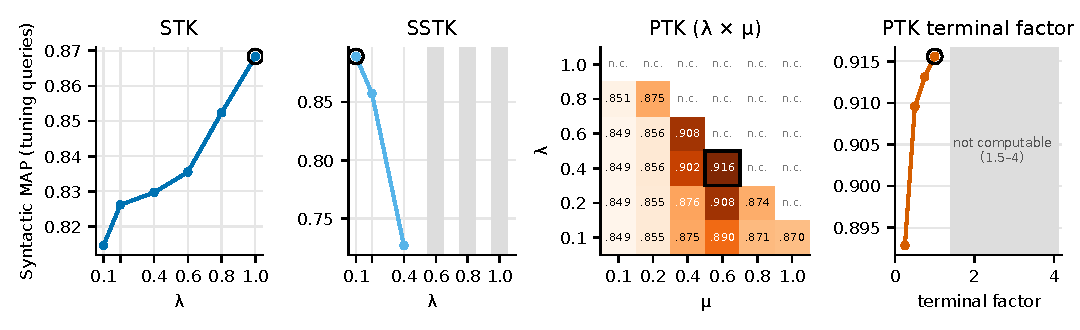
\includegraphics[width=\textwidth]{figures/sensitivity}\caption{Kernel hyper-parameters: MAP for syntactic similarity (mean of the five types) on the 50 tuning queries: STK and SSTK against $\lambda$, PTK over $\lambda \times \mu$ and PTK's terminal factor; circles and the framed cell = the settings used; grey / n.c.\ = not computable.}\label{fig:sensitivity}\end{figure*}


\rqsection{Label noise}{Do the conclusions depend on BigCloneBench's labels?}\label{sec:noise}

\addresses{R1-C3 and R2-C7}

\IfFileExists{tables/noise.tex}{\input{tables/noise}

\begin{figure*}[!htbp]\centering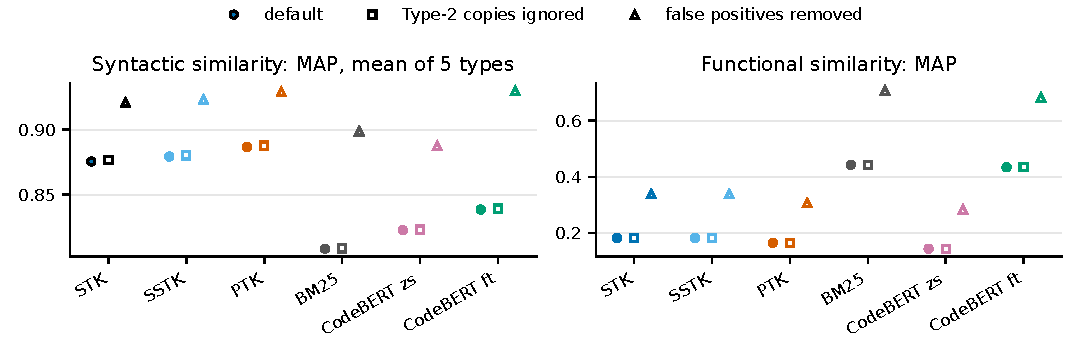
\includegraphics[width=\textwidth]{figures/noise}\caption{Label-noise sensitivity: MAP of each method under the default labels, with Type-2 copies of the query outside its functionality ignored, and with every false positive removed.}\label{fig:noise}
\end{figure*}}{}

We re-scored the rankings of the main evaluation under two alternative labellings. First, ignoring Type-2 copies of the query outside its functionality. Second, removing all
58,103 false positives. Ignoring Type-2 copies changes MAP by at most 0.001 for every method, so mislabeled near-copies do not affect the results.

Removing the false positives raises every method, and it changes one conclusion. For syntactic
similarity, the kernels still lead BM25, but by less (+0.022 to +0.030 instead of +0.067 to +0.078), and they no longer lead fine-tuned CodeBERT ($-$0.009 to $-$0.001 instead of +0.037 to +0.048). Much of the kernels' syntactic advantage therefore comes from ranking BigCloneBench's false positives,
which are lexically similar to the query, below its true clones. 

For functional similarity, the kernels' gap to BM25 and fine-tuned CodeBERT grows (from about $-$0.26 to about $-$0.37 against BM25). The conclusion that the kernels trail both baselines holds under either labeling. 


\rqsection{Diagnostics}{
	How do the trees of large and complex methods differ?}\label{sec:diagnostics}
\addresses{R1-C4}

\noindent RQ3 reports how results change with the size and complexity of the query. This
section looks at the trees themselves, to help explain those changes: it reports the shape of the trees. These
values are computed on the trees of the eligible queries, and are reported as such without statistical tests.
Queries are grouped as in RQ3, by quartile of lines of code (LOC) and by McCabe bin.

\noindent We use these two statements as an example to explain the terms used later in the table:
\begin{center}\scriptsize\begin{tabular}{ll}
\texttt{int i = 0;} & \texttt{(local\_variable\_declaration (integral\_type (int)) (variable\_declarator (ID) (NUM)))} \\ \newline
\texttt{float x = 1;} & \texttt{(local\_variable\_declaration (floating\_point\_type (float)) (variable\_declarator (ID) (NUM)))} \\
\end{tabular}\end{center}
\begin{itemize}
\item \emph{Nodes}: the number of nodes in the tree (6 in each example).
\item \emph{Height}: the number of nodes on the longest path from the root to a leaf (3 in each example).
\item \emph{Branching}: the number of children of a non-leaf node. \emph{Maximum branching} is the largest value in a tree
(2 in each example) and \emph{mean branching} is the average over its non-leaf nodes.
\end{itemize}

\input{tables/d1}

\medskip\noindent\textbf{Tree shape.} This table shows what the trees look like in each size and complexity group, as
the median and interquartile range of each statistic over the group's queries. From the smallest to the largest LOC
quartile, median nodes grow from 79 to 444, height from 10 to 16 and maximum branching from 6 to 14, while mean branching
stays almost constant (1.94 to 1.98). Larger methods therefore have a few nodes with many children, rather than more
branching everywhere.


\medskip\noindent In RQ3, on syntactic similarity, the kernels respond to size in
opposite directions: from the smallest to the largest LOC quartile, PTK's MAP falls from 0.912 to
0.854, whereas STK's rises from 0.875 to 0.925. The tree shape suggests why. Large methods differ
mainly in having a few very wide nodes, such as blocks with many statements, while mean branching
stays constant. PTK matches any subset of a node's children, so a wide node yields very many partial
fragments, many of them generic statement sequences that unrelated methods also contain; these
shared fragments raise the scores of non-clones. STK counts only complete subtrees, so on large
methods it is credited mainly for large, exactly shared structures, which a large method's syntactic
clones have and its non-clones rarely do. 

For functional similarity, every technique declines with
size, BM25 and CodeBERT included (BM25 from 0.557 to 0.322), so this decline is not explained by the trees alone.

%\textbf{Branching.} This table asks whether maximum branching affects PTK and STK differently, since PTK can match parts of a node's children while STK needs complete subtrees. Queries are grouped by quartile of maximum branching, over the eligible queries; the brackets give the lowest and highest maximum branching in each group. The table gives each kernel's MAP and the difference. For syntactic similarity, PTK leads STK at the lowest maximum branching (+0.034 MAP) and trails it at the highest ($-$0.066). For functional similarity, PTK is below STK in every group.
%\input{tables/d3}


%What the SSTK column adds: for functional similarity, SSTK behaves like STK. Its wrong results overlap with the query slightly less than its relevant methods in the smallest quartile (0.38 vs 0.39) and more in the other three. Your Overview paragraph's conclusion therefore holds for all three kernels.

%The Overview paragraph is now partly out of date. It says "for STK and PTK", and the table now has SSTK too. It could become "for PTK and SSTK, the top wrong results overlap ... in all but the smallest", with PTK listed separately since its pattern holds in every group. I haven't changed the text.


\rqsection{Size and complexity}{Do the techniques perform differently on ``small but complex'' and
``large but simple'' methods?}\label{sec:quadrants}
\addresses{R2-C4.}

We split the queries at the median of each measure, 21 lines of code and a McCabe complexity of 4,
which gives four groups from small and simple to large and complex. McCabe's limit of 10 is not used
for this split, because only 10 queries have at most 21 lines and a complexity above 10. The table
gives each method's MAP per group, from the rankings of the main evaluation, without statistical
tests.

\medskip\noindent For the tree kernels, size matters more than complexity. For functional similarity, they do much better on small but complex methods than on large but simple ones (STK 0.204
against 0.116, PTK 0.223 against 0.086), whereas BM25 does slightly better on large but simple ones
(0.446 against 0.420) and fine-tuned CodeBERT, like the kernels, does better on small but complex
ones (0.499 against 0.403). For syntactic similarity, STK and SSTK hardly change across the four
groups (0.867--0.893), PTK is lower on large methods (0.898 and 0.905 on small methods, 0.870 and
0.859 on large ones), and BM25 is higher on large methods (0.883 and 0.903, against 0.745 and 0.833
on small ones).


\input{tables/rq3_quadrants}

		
\rqsection{Effect Sizes and p-values}{What are the effect sizes and p-values of hybrid model comparison?}\label{sec:effects}
\addresses{R2-C5.}

\begin{table*}[!htbp]
\centering
\caption{RQ4 test results. Each hybrid (BM25's top 100 re-ranked by a tree kernel) against its kernel's full ranking, BM25 and fine-tuned CodeBERT. Difference in MAP between hybrid and other model with Bonferroni-adjusted 99.4\% CI and $p$-value (9 comparisons per measure), and effect size $A_{12}$. Bold values indicate that CI excludes 0.}
\label{tab:rq4_tests}
\footnotesize
\setlength{\tabcolsep}{3pt}
\begin{tabular}{lllrrrl}
\toprule
Measure & Hybrid & Against & $\Delta$ MAP & Adjusted CI & Adjusted $p$ & $A_{12}$ \\
\midrule
Mean of types & STK-Hybrid & STK & -0.038 & [-0.071, +0.005] & 0.106 & 0.46 negligible \\
Mean of types & STK-Hybrid & BM25 & \textbf{+0.029} & \textbf{[+0.015, +0.050]} & \textbf{$<$0.002} & 0.56 small \\
Mean of types & STK-Hybrid & CodeBERT ft & -0.001 & [-0.058, +0.048] & 1.000 & 0.50 negligible \\
Mean of types & SSTK-Hybrid & SSTK & -0.042 & [-0.075, +0.002] & 0.079 & 0.46 negligible \\
Mean of types & SSTK-Hybrid & BM25 & \textbf{+0.029} & \textbf{[+0.015, +0.051]} & \textbf{$<$0.002} & 0.56 small \\
Mean of types & SSTK-Hybrid & CodeBERT ft & -0.001 & [-0.057, +0.049] & 1.000 & 0.50 negligible \\
Mean of types & PTK-Hybrid & PTK & -0.049 & [-0.095, +0.006] & 0.122 & 0.45 negligible \\
Mean of types & PTK-Hybrid & BM25 & \textbf{+0.029} & \textbf{[+0.014, +0.052]} & \textbf{$<$0.002} & 0.57 small \\
Mean of types & PTK-Hybrid & CodeBERT ft & -0.001 & [-0.057, +0.051] & 1.000 & 0.50 negligible \\
\midrule
Functional & STK-Hybrid & STK & \textbf{+0.257} & \textbf{[+0.156, +0.382]} & \textbf{$<$0.002} & 0.92 large \\
Functional & STK-Hybrid & BM25 & -0.003 & [-0.013, +0.001] & 0.326 & 0.51 negligible \\
Functional & STK-Hybrid & CodeBERT ft & +0.005 & [-0.045, +0.057] & 1.000 & 0.53 negligible \\
Functional & SSTK-Hybrid & SSTK & \textbf{+0.257} & \textbf{[+0.156, +0.383]} & \textbf{$<$0.002} & 0.92 large \\
Functional & SSTK-Hybrid & BM25 & -0.003 & [-0.013, +0.001] & 0.295 & 0.50 negligible \\
Functional & SSTK-Hybrid & CodeBERT ft & +0.005 & [-0.045, +0.057] & 1.000 & 0.52 negligible \\
Functional & PTK-Hybrid & PTK & \textbf{+0.277} & \textbf{[+0.161, +0.424]} & \textbf{$<$0.002} & 0.91 large \\
Functional & PTK-Hybrid & BM25 & -0.001 & [-0.009, +0.004] & 1.000 & 0.56 small \\
Functional & PTK-Hybrid & CodeBERT ft & +0.008 & [-0.042, +0.061] & 1.000 & 0.53 negligible \\
\bottomrule
\end{tabular}
\end{table*}

We test each hybrid against its kernel's full ranking, BM25 and fine-tuned CodeBERT on MAP, separately
for syntactic similarity (mean of the five clone types) and functional similarity. Queries of the same
functionality are not independent, so we use a paired bootstrap over functionalities (10,000
replicates, with the same resampling for every method). With 9 comparisons per measure, we report
Bonferroni-adjusted 99.4\% percentile CIs and the matching adjusted $p$-values; a difference is
significant when its CI excludes 0. The effect size $A_{12}$ is the share of queries on which the
hybrid ranks better, counting ties as half. nP@5, nP@10 and MRR are reported without tests.



\medskip\noindent For syntactic similarity, every hybrid outperforms BM25 ($\Delta$ MAP $= +0.029$,
$p < 0.002$, $A_{12} = 0.56$--$0.57$, small) and does not differ significantly from its kernel's full
ranking ($-0.038$ to $-0.049$, $p \geq 0.079$) or from fine-tuned CodeBERT ($-0.001$, $p = 1.000$).
Restricting the kernel to BM25's top 100 therefore keeps most of its syntactic effectiveness. For
functional similarity, every hybrid is far above its kernel's full ranking ($+0.257$ to $+0.277$,
$p < 0.002$, $A_{12} = 0.91$--$0.92$, large), because BM25's candidates already contain most of the
relevant methods that the full kernel ranking misses, and it does not differ significantly from BM25
or fine-tuned CodeBERT.
All other effects are negligible, except PTK-Hybrid against BM25 on functional similarity
($A_{12} = 0.56$, small), which is not significant.


	\end{letter}
		\bibliographystyle{plain}
\bibliography{rref}
	

\end{document}




